\chapter{Algorithms}

Graph-based ANNS algorithms are generally separated into two phases: Index construction and Search.

The search phase is very similar across all algorithms. In short, it is simply a \textsc{GreedySearch} algorithm (Algorithm \ref{alg:greedy-search}) modified to fit the specific graph structure. The main difference between algorithms lies in the index construction step---how the graph is constructed and how the vertices inside it are connected.

\section{Search}

\begin{algorithm}[H]
    \caption{\textsc{GreedySearch}(Query \(q\), Starting \(s\), Max candidate size \(L\))}\label{alg:greedy-search}
    \begin{algorithmic}[1]
        \State{\(\mathcal{L} \gets \left\{s\right\}\); \(\mathcal{V} \gets \emptyset\)} \Comment{candidates \(\mathcal{L}\), visited \(\mathcal{V}\)}
        \While{\(\mathcal{L} \setminus \mathcal{V} \neq \emptyset\)}
            \State{\(p^* \gets \arg\min_{p \in \mathcal{L} \setminus \mathcal{V}} \delta(p, q)\)}
            \State{\(\mathcal{L} \gets \mathcal{L} \cup N_{\text{out}}(p^*)\)}
            \State{\(\mathcal{V} \gets \mathcal{V} \cup \left\{p^*\right\}\)}
            \If{\(|\mathcal{L}| > L\)}
                \State{\(\mathcal{L} \gets \textsc{GetClosest}(\mathcal{L}, L)\)}
            \EndIf
        \EndWhile
        \State{\Return{\(\mathcal{L}, \mathcal{V}\)}}
        % \State{Init \(\mathcal{L}\) as work queue with \(s\)}
        % \State{Init \(\mathcal{V}\) to store visited vertices}
        % \While{\(\mathcal{L}\) contains unvisited vertices}
        %     \State{Let \(p^*\) be point closest to \(q\) in \(\mathcal{L}\)}
        %     \State{Add \(N(p^*)\) to \(\mathcal{L}\)}
        %     \State{Mark \(p^*\) as visited}
        %     \If{\(|\mathcal{L}| > L\)}
        %         \State{Pick \(L\) points closest to \(q\) in \(\mathcal{L}\) to keep}
        %     \EndIf
        % \EndWhile
        % \State{\Return{\([\mathcal{L}, \mathcal{V}]\)}}
    \end{algorithmic}
\end{algorithm}

Intuitively, \textsc{GreedySearch} searches for the query \(q\) by first storing a collection of nearest neighbor candidates \(\mathcal{L}\) and a collection of visited vertices \(\mathcal{V}\). Starting from some starting point \(s\) (usually determined by the graph), it greedily picks its neighbors that are closest to \(q\) and traverses the graph until it cannot anymore. 
A visualization of this can be seen in Figure \ref{fig:greedy-viz}.

% For example, consider running \textsc{GreedySearch} with \(L=k=20\) and the neighbors of a vertex are its nearest neighbors. The data set, the starting point \(p\), and the query point \(q\) can be seen in Figure \ref{fig:gs-input}.
% \begin{enumerate}
%     \item Next, the neighbors of \(s\) are added to \(\mathcal{L}\) as shown in Figure \ref{fig:gs1}. Note that red now represents \(\mathcal{V}\) and the first visited point is \(s\).
%     \item Then, the point \(p^*\) in \(\mathcal{L}\) closest to \(q\) (right red point) is visited and its neighbors are added to \(\mathcal{L}\) as shown in Figure \ref{fig:gs2}. Note that since \(L=k\) and every neighbor of \(p^*\) is closer to \(q\) than the previously visited point, \(\mathcal{L}\) is replaced with the neighbors of \(p^*\).
%     \item This is repeated until \textsc{GreedySearch} terminates as shown in Figure \ref{fig:gs3} and \ref{fig:gs4}.
%     \item Finally, the approximate nearest neighbors \(\mathcal{L}\) and the visited vertices---the path from start to query---\(\mathcal{V}\) are returned as shown in Figure \ref{fig:gs-return}.
% \end{enumerate}

\begin{figure}[ht]
    \centering
    \hfill
    \begin{subfigure}{0.31\textwidth}
        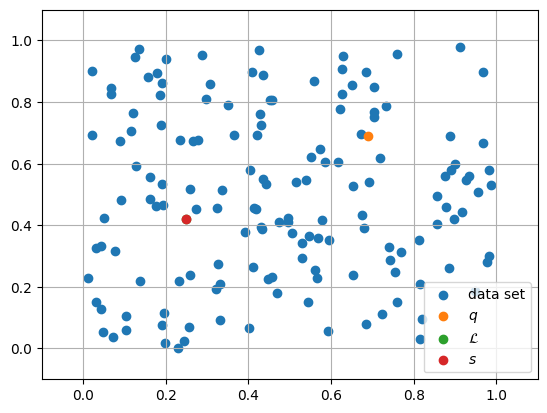
\includegraphics[width=\textwidth]{images/greedy-search-begin}
        \caption{Input}
        \label{fig:gs-input}
    \end{subfigure}
    \hfill
    \begin{subfigure}{0.31\textwidth}
        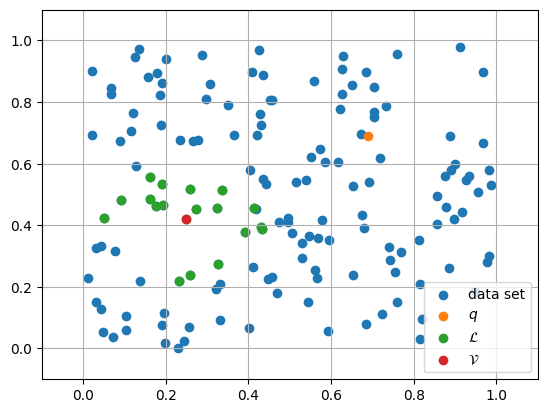
\includegraphics[width=\textwidth]{images/greedy-search-1}
        \caption{Iteration 1}
        \label{fig:gs1}
    \end{subfigure}
    \hfill
    \begin{subfigure}{0.31\textwidth}
        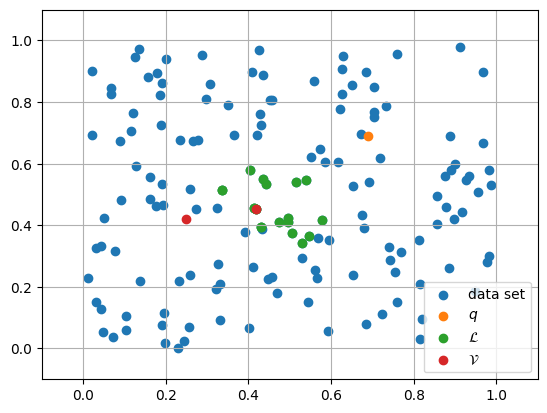
\includegraphics[width=\textwidth]{images/greedy-search-2}
        \caption{Iteration 2}
        \label{fig:gs2}
    \end{subfigure}
    \hfill

    \hfill
    \begin{subfigure}{0.31\textwidth}
        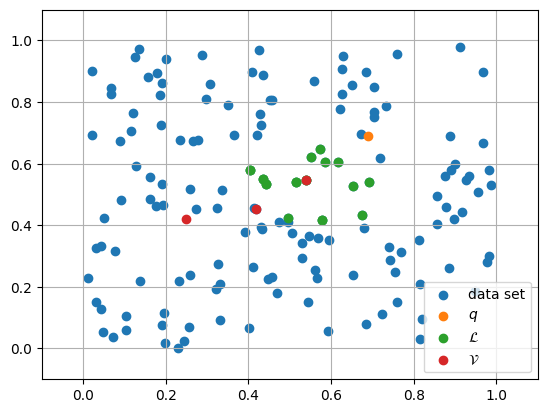
\includegraphics[width=\textwidth]{images/greedy-search-3}
        \caption{Iteration 3}
        \label{fig:gs3}
    \end{subfigure}
    \hfill
    \begin{subfigure}{0.31\textwidth}
        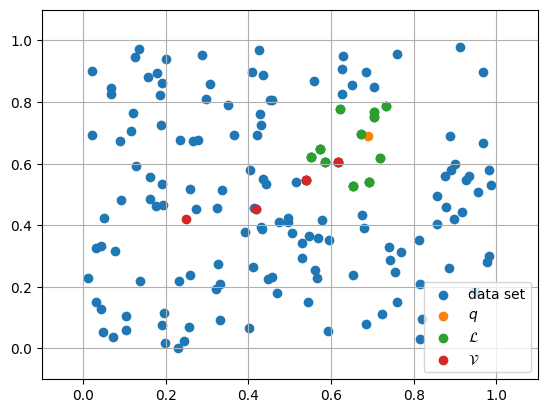
\includegraphics[width=\textwidth]{images/greedy-search-4}
        \caption{Iteration 4}
        \label{fig:gs4}
    \end{subfigure}
    \hfill
    \begin{subfigure}{0.31\textwidth}
        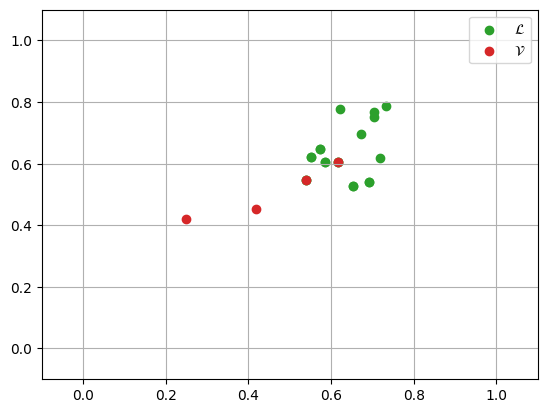
\includegraphics[width=\textwidth]{images/greedy-search-final}
        \caption{Returning values}
        \label{fig:gs-return}
    \end{subfigure}
    \hfill
    \caption{Visualization of \textsc{GreedySearch}}
    \label{fig:greedy-viz}
\end{figure}

\section{Index Construction}

Similar to the search phase, the index construction phase has similar flows across algorithms as well. The general flow can be seen in Algorithm \ref{alg:build-index}.

\begin{algorithm}[H]
    \caption{\textsc{BuildIndex}(Data \(\mathcal{P}\), Start point \(s\), Beam width \(L\), Degree bound \(M\))}
    \label{alg:build-index}
    \begin{algorithmic}[1]
        \For{\(p \in \mathcal{P}\)}
            \State{Add \(p\) to graph}
            \State{\([\mathcal{L}, \mathcal{V}] \gets \textsc{GreedySearch}(p, s, L, 1)\)} \Comment{Searches for \(p\) in existing graph}
            \State{\(N(p) \gets \textsc{Prune}(p, \mathcal{V})\)}
        \EndFor
    \end{algorithmic}
\end{algorithm}

Intuitively, the algorithm adds the point \(p\) into the graph as a vertex, runs a search to \(p\), and assigns the \textit{path} from the starting point \(s\) to \(p\) after it has been pruned using the heuristic determined by the graph.

\section{HNSW and DiskANN}

Since vertex removal should not degrade the performance and quality of the graph, it is better to design the removal algorithm on top of an existing algorithm that already performs well instead of starting from scratch. Among the existing graph-based ANNS algorithms, Hierarchical Navigable Small World (HNSW) \cite{hnsw} and DiskANN \cite{diskann-paper} are two of the best performing ones. That is, at a fixed target accuracy level, they are able to answer high number of queries per second (QPS) \cite{annscaling,survey2} while having comparable or better build times compared to other graph-based algorithms \cite{annscaling}.

\begin{figure}[ht]
    \centering
    \hfill
    \begin{subfigure}{0.45\textwidth}
        \centering
        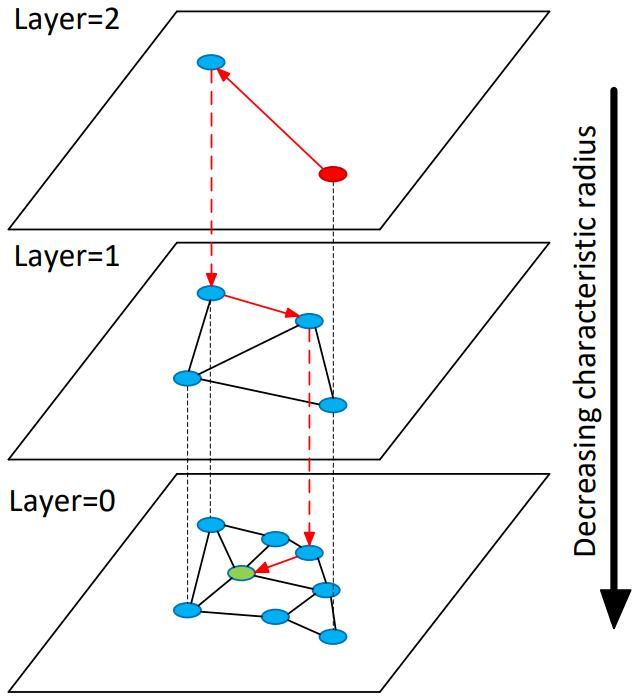
\includegraphics[height=0.2\textheight]{images/hnsw}
        \caption{HNSW \cite{hnsw}}
        \label{fig:hnsw-viz}
    \end{subfigure}
    \hfill
    \begin{subfigure}{0.45\textwidth}
        \centering
        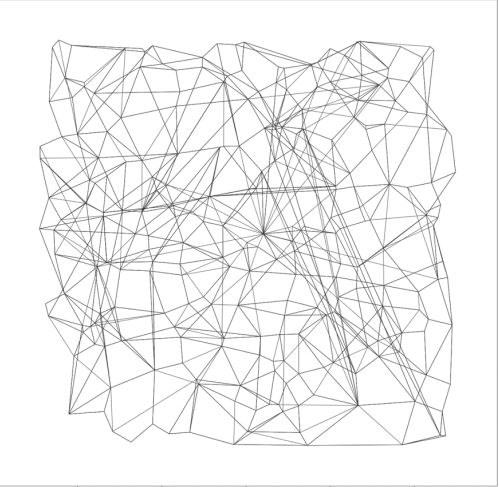
\includegraphics[height=0.2\textheight]{images/diskann}
        \caption{DiskANN \cite{diskann-paper}}
        \label{fig:diskann-viz}
    \end{subfigure}
    \hfill
    \caption{Visualization of existing, best-performing algorithms}
\end{figure}

\subsection{Hierarchical Navigable Small World (HNSW)}

As shown in Figure \ref{fig:hnsw-viz}, HNSW is a multi-layer graph where the points are \textit{promoted} and cloned to higher layers based on exponentially decaying probability. That is, the probability makes it so that fewer points show up in higher layers.

HNSW constructs its graph incrementally by adding the points to the graph one-by-one. The construction first decides which layer the new point belongs to and run Algorithm \ref{alg:build-index} on each layer from top to bottom. As for its pruning criteria, it ensures that there is a small, circular radius around the new point. The search is done on every layer but the \(k\) nearest neighbors are only picked from the lowest layer.

% \begin{algorithm}[H]
% \caption{SelectNeighbors Algorithm}\label{alg:select-nbrs}
% \begin{algorithmic}[1]
%     \Function{SelectNeighbors}{\(G, q, \mathcal{C}, M\){}}
%         \State{\(\mathcal{R} \gets \emptyset\); \(\mathcal{W} \gets \mathcal{C}\)} \Comment{keepers \(\mathcal{R}\), candidates \(\mathcal{W}\)}
%         \While{\(|\mathcal{W}| > 0\) and \(|\mathcal{R}| < M\)}
%             \State{\(p^* \gets \arg\min_{p \in \mathcal{W}} \delta(p, q)\)}
%             \If{\(\delta(p^*, q) < \min_{p' \in \mathcal{R}} \delta(p', q)\)}
%                 \State{\(\mathcal{R} \gets \mathcal{R} \cup \left\{e\right\}\)}
%             \EndIf
%         \EndWhile
%         \State{\Return{\(\mathcal{R}\)}}
%     \EndFunction
% \end{algorithmic}
% \end{algorithm}

% \textbf{Inputs:} Graph \(G\), Query \(q\), Candidates \(\mathcal{C}\), Max degree \(M\)



% \begin{algorithm}[H]
% \caption{HNSW Algorithm}\label{alg:hnsw}
% \begin{algorithmic}[1]
%     \Function{HNSW}{\(\mathcal{P}, C, M, m_L\)}
%         \State{\(G \gets\) empty graph}
%         \For{\(p \in \mathcal{P}\)}
%             \State{\(\mathcal{W} \gets \emptyset\), \(ep \gets s\)}
%         \EndFor
%         \State{\Return{\(G\)}}
%     \EndFunction
% \end{algorithmic}
% \end{algorithm}

% \textbf{Inputs:} Point set \(\mathcal{P}\)

\subsection{DiskANN}

DiskANN works in a similar way to HNSW but in a single layer. As shown in Figure \ref{fig:diskann-viz}, it constructs a graph with both short and long edges within a single layer and the connections spread out from the center of the graph which is the starting point.

The construction is rather simple. It is essentially Algorithm \ref{alg:build-index} with the medoid of the data set being the starting point. The pruning criteria ensures that the points in the path from the starting point to the new point are not too close to each other. The search is essentially Algorithm \ref{alg:greedy-search} starting from the medoid.

% \begin{algorithm}[H]
% \caption{RobustPrune Algorithm}\label{alg:robust-prune}
% \begin{algorithmic}[1]
%     \Procedure{RobustPrune}{\(G, p, \mathcal{V}, \alpha, M\){}}
%         \State{\(\mathcal{V} \gets \mathcal{V} \cup N_{\text{out}}(p) \setminus \left\{p\right\};N_\text{out}(p) \gets \emptyset\)}
%         \While{\(\mathcal{V} \neq \emptyset\)}
%             \State{\(p^* \gets \arg\min_{p \in \mathcal{V}} \delta(p, q)\)}
%             \State{\(N_\text{out}(p) \gets N_\text{out}(p) \cup \left\{p^*\right\}\)}
%             \If{\(|N_\text{out}(p) = M\)}
%                 \State{break}
%             \EndIf
%             \For{\(p' \in \mathcal{V}\)}
%                 \If{\(\alpha \cdot \delta(p^*, p') \leq \delta(p, p')\)}
%                     \State{\(\mathcal{V} \gets \mathcal{V} \setminus \left\{p'\right\}\)}
%                 \EndIf
%             \EndFor
%         \EndWhile
%     \EndProcedure
% \end{algorithmic}
% \end{algorithm}

% \textbf{Inputs:} Graph \(G\), Starting point \(p\), Candidate set \(\mathcal{V}\), Distance scaler \(\alpha\), Max degree \(M\)

% \begin{algorithm}[H]
% \caption{Vamana Algorithm}\label{alg:vamana}
% \begin{algorithmic}[1]
%     \Function{Vamana}{\(\mathcal{P}, \alpha, C, M\){}}
%         \State{Initialize \(G\) as random directed graph with max degree \(M\)}
%         \State{\(s \gets \textsc{Medoid}(\mathcal{P})\); \(n \gets |\mathcal{P}|\)}
%         \For{\(p \in \mathcal{P}\)}
%             \State{\(\mathcal{L}, \mathcal{V} \gets \textsc{GreedySearch}(s, p, 1, C)\)}
%             \State{\(\textsc{RobustPrune}(p, \mathcal{V}, \alpha, M)\)}
%             \For{\(p' \in N_\text{out}(p)\)}
%                 \If{\(|N_\text{out}(p') \cup \left\{p'\right\}| > M\)}
%                     \State{\(\textsc{RobustPrune}(p', N_\text{out}(p')\cup\left\{p'\right\}, \alpha, M)\)}
%                 \Else
%                     \State{\(N_\text{out}(p') \gets N_\text{out}(p') \cup \left\{p'\right\}\)}
%                 \EndIf
%             \EndFor
%         \EndFor
%         \State{\Return{\(G\)}}
%     \EndFunction
% \end{algorithmic}
% \end{algorithm}

% \textbf{Inputs:} Point set \(\mathcal{P}\), Dist. scaler \(\alpha\), Candidate size \(C\), Max degree \(M\)

\subsection{Similarities and Differences}

A common pattern that shows up in both algorithms is the concept of long and short edges. In short, long edges allows for the algorithm to traverse from the starting point to the query point very quickly and the short edges allow for \textit{fine-tuning} the results.

However, the structure of the graph and its construction algorithm are slightly different. Namely, HNSW is a multi-layer undirected graph while DiskANN is a single-layer directed graph. Their pruning heuristics (line 4 in Algorithm \ref{alg:build-index}) are also different.
